\documentclass[times, utf8, zavrsni, numeric]{fer}
\usepackage{booktabs}

\begin{document}

% TODO: Navedite broj rada.
\thesisnumber{1160}

% TODO: Navedite naslov rada.
\title{Algoritmi za brzo učenje na neprijateljskim primjerima}

% TODO: Navedite vaše ime i prezime.
\author{Dominik Jambrović}

\maketitle

% Ispis stranice s napomenom o umetanju izvornika rada. Uklonite naredbu \izvornik ako želite izbaciti tu stranicu.
% \izvornik

% Dodavanje zahvale ili prazne stranice. Ako ne želite dodati zahvalu, naredbu ostavite radi prazne stranice.
% \zahvala{}

\tableofcontents

\chapter{Uvod}
Velik broj problema s kojima se danas susrećemo takve su prirode da ne znamo kako ih riješiti koristeći klasičan, algoritamski pristup. Razlog tome često leži u činjenici da ne znamo ni kako mi sami rješavamo te probleme, 
a jedan od najčešćih primjera za to je raspoznavanje tj.\ klasifikacija slika.
Jedno od mogućih rješenja takvih problema je korištenje umjetnih neuronskih mreža - mreža sastavljenih od velikog broja povezanih jedinica (neurona) koje obavljaju veoma jednostavne operacije.

Razvojem dubokih neuronskih mreža došlo je do ubrzanog napretka u području računalnog vida. Računalni vid područje je umjetne inteligencije koje se bavi problemima poput klasifikacije 2D slika. 
Sve većom popularizacijom i korištenjem dubokih modela u sustavima različitih namjena, u pitanje se dovodi sigurnost takvih modela -
ako model želimo koristiti u automobilima s ciljem detekcije pješaka i vozila, model mora moći dobro generalizirati, kao i biti robustan. Takav model ne bi smio mijenjati svoje odluke na temelju veoma malih promjena na ulazu -
na primjeru prometa, želimo da model točno detektira pješaka, bez obzira nosi li on kapu ili ne.

Kako bi ostvarili robustnost modela, predložene su brojne tehnike, a jedna od najpopularnijih je robusno učenje tj.\ učenje na neprijateljskim primjerima. 
Kada su u pitanju modeli koji brzo uče, robusno učenje prihvatljivo je rješenje za postizanje robusnih modela otpornih na napade. 
Ipak, kada su u pitanju veći modeli za koje učenje traje veoma dugo, obično robusno učenje često je neprihvatljivo. 
U tu svrhu, razvijene su metode koje ubrzavaju robusno učenje. U ovome radu, razmatrat ćemo tri takve metode: besplatno robusno učenje~\cite{shafahi2019adversarial}, brzo robusno učenje~\cite{wong2020fast} i
nadogradnju na brzo robusno učenje (FastAdv+ i FastAdvW,~\cite{li2020towards}). 

Uz to, razmatrat ćemo i otpornost naučenih modela na zatrovane podatke. Zatrovani podatci ulazi su izmijenjeni s ciljem navođenja modela na neočekivano ponašanje. 
Uvođenjem takve ranjivosti u model, napadači mogu neprimjećeno postići proizvoljne ciljeve poput izbjegavanja detekcije ili pogrešne klasifikacije.

\chapter{Neuronske mreže}
\section{Općenito o neuronskim mrežama}
Umjetne neuronske mreže veoma su popularan alat za rješavanje kompleksnih problema za koje je teško modelirati ili formalizirati znanje. 
Predstavnik su konektivističkog pristupa umjetnoj inteligenciji~\cite{uui2020} koji se zasniva na oblikovanju sustava inspiriranih građom mozga.

Problemi koje rješavamo umjetnim neuronskim mrežama svrstavaju se u dvije glavne kategorije:
\begin{enumerate}
    \item klasifikacija 
    \item regresija
\end{enumerate}

Da bi neuronska mreža mogla rješavati takve probleme, važno nam je da može učiti na temelju predočenih podataka. Učenje neuronske mreže odvija se izmjenom težina pojedinih neurona (time znanje implicitno ugrađujemo u našu mrežu).
Kako bismo detaljnije mogli govoriti o učenju i arhitekturama neuronskih mreža, važno je ukratko opisati neuron - osnovnu gradivnu jedinicu svake mreže.
\pagebreak
\section{Umjetni neuron}
Umjetni neuroni predstavljaju jednostavne procesne jedinice koje modeliraju ponašanje prirodnih neurona. Osnovni neuron akumulira vrijednosti na ulazu pomnožene težinama, 
akumuliranoj vrijednosti dodaje pomak te na kraju istu propušta kroz prijenosnu (aktivacijsku) funkciju. Ponašanje jednog neurona možemo modelirati jednadžbom

\begin{equation}
    o = f(\sum_{i=1}^{n}x_{i} * w_{i} + b)
    \label{eq:neuron}
\end{equation}
\\
\noindent pri čemu x označava pojedine ulaze, w težine na pripadnim ulazima, b pomak te f prijenosnu funkciju. 

\section{Prijenosne funkcije}
Neki od najranijih modela umjetnog neurona kao prijenosnu funkciju koristili su funkciju identiteta (ADELINE-neuron) te funkciju skoka (TLU-perceptron).
S vremenom su korištene i razvijene brojne druge prijenosne funkcije poput sigmoidalne funkcije definirane kao 

\begin{equation}
    sigmoid(net) = \frac{1}{1 + e^{-net}}
    \label{eq:sigmoid}
\end{equation}
\\
\noindent i zglobnice (ReLU - engl.\ \textit{Rectified Linear Unit}) definirane kao

\begin{equation}
    relu(net) = max(0, net)
    \label{eq:relu}
\end{equation}
\\
\noindent Važno je primijetiti da ako je prijenosna funkcija linearna, cijeli neuron može postići isključivo linearnu transformaciju. 
Kako bi umjetnim neuronima mogli modelirati kompleksnije funkcije, koristimo nelinearne prijenosne funkcije poput sigmoidalne funkcije i zglobnice. 
Pritom je za duboke neuronske mreže s velikim brojem slojeva često korištena upravo zglobnica - 
sigmoidalna funkcija za takve mreže nije prikladna zbog problema nestajućeg gradijenta (engl.\ \textit{vanishing gradient problem}) koji nastaje tijekom učenja temeljenog na gradijentnim metodama.

\section{Arhitektura umjetne neuronske mreže}
Kada je za neki problem potrebno koristiti više od jednog osnovnog neurona, neurone povezujemo u mrežu. Pritom kažemo da se neuronska mreža sastoji od nekolicine slojeva:
\begin{enumerate}
    \item ulazni sloj
    \item skriveni slojevi
    \item izlazni sloj
\end{enumerate}
Iako ulazni sloj predstavljamo neuronima, oni, za razliku od neurona u skrivenim slojevima i izlaznom sloju, ne obavljaju nikakve transformacije - možemo reći da predstavljaju ulazni podatak.
Veličina ulaznog sloja govori nam o dimenzionalnosti ulaznih podataka, a veličina izlaznog sloja u slučaju problema klasifikacije često nam govori o broju razreda u koje klasificiramo ulaz. 

\begin{figure}[htb]
    \centering
    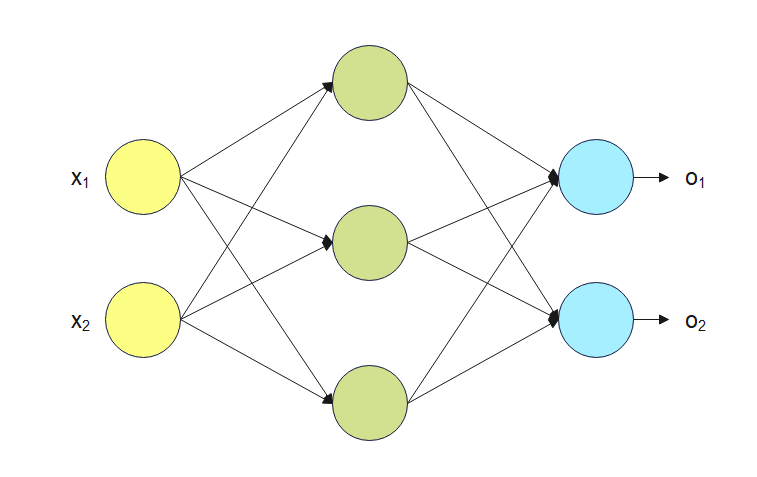
\includegraphics{basic_nn_labeled.png}
    \caption{2x3x2 arhitektura umjetne neuronske mreže}
    \label{fig:basic_nn}
\end{figure}

Na slici~\ref{fig:basic_nn} moguće je vidjeti primjer arhitekture umjetne neuronske mreže. 
Neuroni označeni žutom bojom predstavljaju ulazni sloj, neuroni označeni zelenom bojom skriveni sloj, a neuroni označeni plavom bojom izlazni sloj. 
Ovakvu arhitekturu mreže skraćeno možemo označiti kao 2x3x2 neuronsku mrežu. Pritom brojke označavaju broj neurona u pojedinom sloju (ulazni sloj je prvi sloj mreže).

Za ovakvu mrežu kažemo da je unaprijedna potpuno-povezana mreža. 
Pojam unaprijedna mreža označava to da ne postoje veze iz dubljih slojeva prema plićim slojevima, a pojam potpuno-povezana mreža označava to da svaki neuron ima vezu sa svakim neuronom iz prethodnog sloja.
Uz to, svi neuroni imaju i dodatnu težinu zvanu pomak (nije prikazano na slici ~\ref{fig:basic_nn}). Djelovanje jednog sloja mreže sažeto možemo prikazati kao

\begin{equation}
    \pmb{h}_{i} = f(\pmb{W}_{i} * \pmb{h}_{i-1} + \pmb{b}_{i})
    \label{eq:nn_layer}
\end{equation}
\\
pri čemu W\textsubscript{i} predstavlja težine trenutnog sloja, b\textsubscript{i} pomake trenutnog sloja, h\textsubscript{i-1} izlaz iz prethodnog sloja, f prijenosnu funkciju primijenjenu na svaki element te h\textsubscript{i} izlaz iz trenutnog sloja.
Korištenjem takve formule za svaki sloj mreže, na kraju ćemo dobiti izlaz mreže za neki proizvoljni ulaz. Ovo nazivamo unaprijednim prolazom.

\section{Učenje neuronske mreže}
Kako bismo mogli koristiti proizvoljnu mrežu za probleme klasifikacije ili regresije, potrebno ju je prvo naučiti. 
Kao što je već prethodno rečeno, učenje neuronske mreže odgovara izmjeni težina pojedinih neurona, a najčešće se postiže algoritmom propagacije pogreške unatrag~\cite{Goodfellow-et-al-2016}.
Da bismo mogli znati kako trebamo izmijeniti težine neurona, prvo trebamo znati koliko naš model griješi. Mjera greške naziva se gubitak, a računa se na temelju izlaza modela i očekivanog (točnog) izlaza.
Za izračun gubitka često je korištena unakrsna entropija koju možemo definirati kao

\begin{equation}
    H(P^{*}|P) = -\sum_{i}P^{*}(i) * \log{P(i)}
    \label{eq:cross_entropy}
\end{equation}
\\
pri čemu P\textsuperscript{*}(i) označava distribuciju očekivanog izlaza, a P(i) distribuciju izlaza modela.
Jednom kada znamo iznos gubitka, računajući iznos gradijenta funkcije gubitka (parcijalne derivacije gubitka po težinama) isti možemo upotrijebiti za izmjenu iznosa težina koristeći gradijentni spust. 
Iterativnim ponavljanjem ovakvog postupka minimiziramo iznos funkcije gubitka, time dobivajući što bolju mrežu.

\pagebreak

Nakon učenja mreže na skupu za učenje, evaluirat ćemo performanse mreže na neviđenom skupu zvanom skup za testiranje (engl.\ \textit{test set}). Često korištena mjera za kvalitetu modela je točnost definirana kao

\begin{equation}
    accuracy = \frac{correct}{total}
    \label{eq:accuracy}
\end{equation}
\\
pri čemu correct označava broj točno klasificiranih primjera, total ukupan broj primjera, a accuracy točnost.
Uz točnost, postoje i brojne druge mjere kvalitete modela. Neke od njih su preciznost (engl.\ \textit{precision}), odziv (engl.\ \textit{recall}) i matrica zabune (engl.\ \textit{confusion matrix}).

\section{Duboke neuronske mreže}
Ako želimo rješavati složenije probleme koristeći umjetne neuronske mreže sa samo jednim skrivenim slojem, suočit ćemo se s problemom - broj neurona potreban kako bi umjetna neuronska mreža mogla obavljati svoju zadaću bit će prevelik.
Uz to, korištenjem širokog modela s velikim brojem neurona u skrivenom sloju teško ćemo postići svojstvo generalizacije jer će se model lako prenaučiti i zapamtiti ulazne podatke. 

Zbog tih razloga, veoma su popularne duboke neuronske mreže~\cite{Goodfellow-et-al-2016}. Duboke neuronske mreže, za razliku od mreža sa samo jednim skrivenim slojem, imaju nekolicinu skrivenih slojeva. 
Pritom za rješavanje složenijih problema duboke mreže trebaju imati značajno manje neurona po sloju naspram mreže sa samo jednim skrivenim slojem. 
Zasebni slojevi mreže naučit će prepoznavati zasebne značajke ulaza, a njihovom kombinacijom mreža će moći postići uspješnu klasifikaciju.

Ipak, postoje i određene mane dubokih neuronskih mreža. Jedna od mana činjenica je da je za propagaciju pogreške unazad kod ovakvih mreža potrebno množiti gradijente. 
U slučaju da kao prijenosnu funkciju koristimo sigmoidalnu funkciju, ovo lako vodi do problema nestajućeg gradijenata zbog kojega težine neurona u plitkim slojevima nećemo moći ispravno izmijeniti.
Uz problem nestajućeg gradijenta, postoji i problem eksplodirajućeg gradijenta (engl.\ \textit{exploding gradient problem}) koji se pojavljuje kod nekih drugih prijenosnih funkcija od kojih je najpoznatija upravo zglobnica (ReLU).
Još jedna mana dubokih neuronskih mreža činjenica je da kako bismo kvalitetno naučili duboku mrežu moramo imati veoma velik skup podataka.

\chapter{Konvolucijske duboke neuronske mreže}

\chapter{Zaključak}
Zaključak.

\bibliography{literatura}
\bibliographystyle{fer}

\begin{sazetak}
Sažetak na hrvatskom jeziku.

\kljucnerijeci{Ključne riječi, odvojene zarezima.}
\end{sazetak}

% TODO: Navedite naslov na engleskom jeziku.
\engtitle{Algorithms for fast robust training on adversarial examples}
\begin{abstract}
Abstract.

\keywords{Keywords.}
\end{abstract}

\end{document}
